\subsection{Design Av Dokumentdatabase}
Her brukte vi datasettet "Socio-Economic Country Pofiles" fra Kaggle:

https://www.kaggle.com/nishanthsalian/socioeconomic-country-profiles


\textbf{Hvorfor kolonnedatabase?}

I hovedårsak er det gunstig å bruke dokument-orientert database med dette settet da vi kun trenger å organisere basert på land, og vil gjøre svært få kall mot databasen. Aggregeringene våre kan i flere tilfeller da ligge som referanser i hvert land, og vil heller eksistere som sine egne dokumenter. Ved endringer i datasettet vil aggregeringer kjøres på nytt, og endre verdiene i disse dokumentene. Grunnen til at dette kan være til fordel er hvor tungt det fort blir med mange kall mot dokument-orienterte databaser, så det viktigste blir konsistens på dataen. Når data oppdateres i her vil kun dokumentene som er påvirket av endringene ha operasjoner utført på de.

Mange aggregeringer er også mye raskere å få gjort i denne typen database da man henter ut et helt dokument ved spørringen, og alt informasjonen den inneholder. Dette gjør at man slipper å gjøre søk på tvers av tabeller eller må gjøre mere komplekse nøstede spørringer. I tillegg er det en veldig god modell for databaser som ikke gjør veldig mange endringer ofte, hvor tilgang til replika versjoner av data gir redundans ved mange spørringer og holder ytelsen oppe.

En av de aller mest interessante delene av denne typen database er indeksering, og hvordan det kan brukes for å gjøre at spørringer blir mye billigere. Indeksering tillater også da å lagre spørringer rett i RAM, men det krever at man har plass til hele settet man arbeider med også. I vår aggregering som tar inn brukerspesifiserte land og sammenligner kostnad kan potensielt være større da den kun trenger å holde det nyeste resultatet fra hver spørring.

\textbf{Country-Dokument}

\begin{itemize}
  \item Country: “CountryName”
  \item Population In Thousands: float
  \item GDP: float
  \item GDP Per capita: percent
  \item Unemployment: percent
  \item Labour Force Participation By Gender: percent
  \item PopGrowthRate Annual: Percentage
  \item Urban population: percent
  \item Urban population growth: avg annual precent%
  \item Health Total Expenditure: percent of GDP
  \item Education Total Expenditure: percent of GDP
  \item Education enrollment primary/secondary/tertiary: F/M per 100 pop
  \item Individuals using the internet: per 100 inhabitants
  \item CO2 emission estimates: million tons/tons per capita
  \item Pop. Using improved drinking water: Urban/rural %
  \item Quality of Life Index: float
  \item Purchasing power index: float
  \item Safety Index: float
  \item Health Care Index: int
  \item Cost of Living: float
  \item Cost of living index: float
  \item Property price to income Ratio: float
  \item Affordability index: float
  \item Cost of living plus rent index: float
  \item Life expectancy total: float
  \item Military expenditure: float
  \item Tax revenue: percent of GDP
\end{itemize}

\subsubsection{Aggregeringer}
% Aggregering 1 %
\textbf{Hva er verdens høyeste beskattende land etter GDP.}

Denne aggregeringen kan bli lagret i databasen som et eget dokument da det ikke er noe som endrer seg ofte. Dette gjør det lett å hente ut tabellen, og heller flere redundanskopier av dokumentet gjør at det blir lett tilgjengelig selv ved høy trafikk i databasen.

\FigureCounter
\begin{figure}[H]
  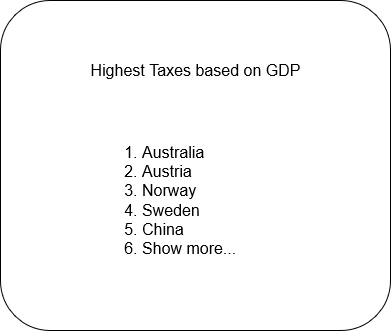
\includegraphics[scale=1]{images/milepael3/highestTaxesByGDP.png}
\end{figure}

\textbf{Pseudo-Kode}
\begin{enumerate}
  \item Hent ut alle land med skatt og GDP
  \item Sorter etter stor del av GDP som blir beskattet
  \item Post (legg inn referanse til aggregering i Land dokumenter)
\end{enumerate}

% Aggregering 2 %
\textbf{Livskvalitet etter skatt}

Denne aggregeringen er en av de mer komplekse vi har, denne spørringen gjøres mot en Multikey Index i landsdokumentene som gjør at den kun trenger å gjøre denne spørringen når data endrer seg. Alternativt kan spørringen lagres som et eget dokument med referanse til landene. Å lagre til dokument kan potensielt være billigere da man heller kan hente ut dette ved hver read, men å indeksere vil gjøre at færre interaksjoner vil skje med unødvendige dokumenter.

\FigureCounter
\begin{figure}[H]
  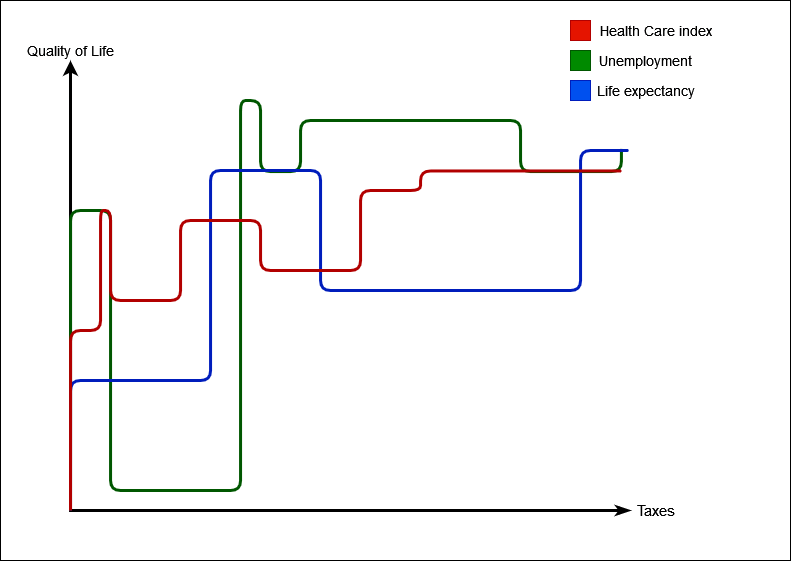
\includegraphics[scale=0.5]{images/milepael3/qualityOfLifeByTaxes.png}
\end{figure}

\textbf{Pseudo-Kode}
\begin{enumerate}
  \item Lag indeks
  \item Hent alle land sine quality of life verdier
  \item Lag objekter med disse verdiene
  \item Legg de sortert i en liste etter skatt i landet
  \item Post til dokument og legg referanse til referanse
\end{enumerate}

% Aggregering 3 %
\textbf{Land sammenlignet etter kost}

Denne aggregeringen er veldig billig ytelsesmessig med kun databasekall for å hente ut landene som blir valgt i menyene. Vi kan da kun sette nødvendige dokumenter i aggregeringspipelinen. Disse landene (…Y) kan da sjekkes mot verdien satt i hovedland(X), og så postes med riktig streng verdi. Dette kan gjøres via On-Demand Materialized Views.

Her vil det bli kjørt da n+1 spørringer mot databasen hvor n = antall Y. Det vil så bli aggregert fra pipeline som en array.

For denne spørringen gir det mening å bruke en indeks som har referanse til alle landsdokumentene. Å bruke indekser gjør at vi heller ser kun på dokumentene vi ønsker, i stedet for at alle dokumentene i samlingen må sjekkes.

\FigureCounter
\begin{figure}[H]
  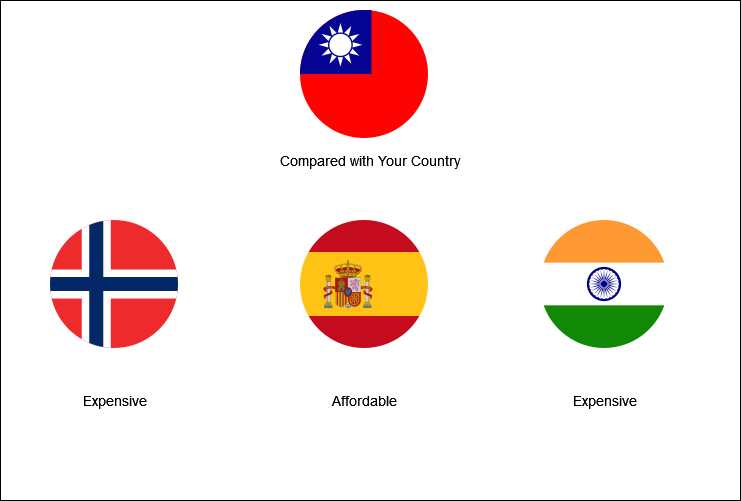
\includegraphics[scale=0.5]{images/milepael3/countriesComparedByExpensiveness.png}
\end{figure}
Denne aggregeringen tar for seg utvalgt land, og sammenligner hvor dyrt det er å bo der, eller reise dit, i forhold til andre populære destinasjoner.

\textbf{Pseudo-Kode}
\begin{enumerate}
  \item Hent alle land og legg de i en liste
  \item Hent valgte lands navn og affordability index
  \item Hvis X sitt land er innen samme verdisone som Y = affordable
  \item Under = cheap
  \item Mer = expensive
  \item Post aggregering
\end{enumerate}

\subsubsection{Endring i data}
\begin{enumerate}
  \item Ny data kommer inn
  \item Landsdokumentene som blir påvirket vil endre informasjon
  \begin{itemize}
    \item Dokument-orienterte databaser vil kun gjøre endringer i dokumenter som blir påvirket av ny data, dersom det har skjedd endringer mot data som har vært indeksert vil det som regel være nødvendig å gjenskape indeksen
  \end{itemize}
  \item Aggregeringer og indekser som påvirkes og er lagret som dokument kjøres og lages på nytt
  \begin{itemize}
    \item Dette blir noe av det dyrere som skjer da aggregeringene kan gjøre mange databasekall, men dette vil være avhengig av hvor mange dokument som skal endres,
    og om endringene som er gjort påvirker de faktiske aggregeringene.
  \end{itemize}
  \item Id feltet vil måtte være det første feltet i en dokument, og rekkefølgen på feltene i objektet vil alltid være det samme så lenge en av endringene som skjer ikke omdøping av felt-navnene 
\end{enumerate}